%\documentclass[landscape,a0b,final,a4resizeable]{a0poster}
%\documentclass[portrait,a0b,final]{a0poster}
\documentclass[portrait,a0b,final]{a0poster}
%\documentclass[orientation=landscape,size=a0,scale=1,final]{a0poster}
%\documentclass[final]{beamer}
%\mode<presentation>
%{
%\usepackage[orientation=landscape,size=a0,scale=1.4,debug]{beamerposter}
%\documentclass[portrait,a0b,final,a4resizeable]{a0poster}
%\documentclass[portrait,a0b,final]{a0poster}
%%% Option "a4resizeable" makes it possible ot resize the
%   poster by the command: psresize -pa4 poster.ps poster-a4.ps
%   For final printing, please remove option "a4resizeable" !!

%\usepackage[ruled,lined]{algorithm2e}
%\def\algorithmautorefname{Algorithm}
%\SetKwIF{If}{ElseIf}{Else}{if}{then}{else if}{else}{endif}

\usepackage{amssymb,amsfonts,amsmath,latexsym,amsthm}
\usepackage[usenames,dvipsnames]{color}
\usepackage{enumitem}
%\theoremstyle{plain}
\newtheorem{theorem}{Theorem}[section]
\newtheorem{corollary}[theorem]{Corollary}
\newtheorem{lemma}[theorem]{Lemma}
\newtheorem{proposition}[theorem]{Proposition}
\newtheorem{condition}[theorem]{Condition}
\newtheorem{algorithm}[theorem]{Algorithm}

\newcommand{\clusters}{\bm{\kappa}}
\newcommand{\cluster}[1]{\kappa_{#1}}
\newcommand{\sizes}{\bm{\mu}}
\newcommand{\size}[1]{\mu_{#1}}
\newcommand{\edist}{\bm{\gamma}}
\newcommand{\shape}{\eta}
\newcommand{\rate}{s}
\newcommand{\betaA}{u}
\newcommand{\betaB}{v}


% Probability distributions
\DeclareMathOperator*{\Exp}{Exp}
\DeclareMathOperator*{\TExp}{TExp}
\DeclareMathOperator*{\Bernoulli}{Bernoulli}
\DeclareMathOperator*{\Beta}{Beta}
\DeclareMathOperator*{\Ga}{Gamma}
\DeclareMathOperator*{\TGamma}{TGamma}
\DeclareMathOperator*{\Poisson}{Poisson}
\DeclareMathOperator*{\Binomial}{Binomial}
\DeclareMathOperator*{\NormalGamma}{NormalGamma}
\DeclareMathOperator*{\InvGamma}{InvGamma}
\DeclareMathOperator*{\Cauchy}{Cauchy}
\DeclareMathOperator*{\Uniform}{Uniform}
\DeclareMathOperator*{\Gumbel}{Gumbel}
\DeclareMathOperator*{\Pareto}{Pareto}
\DeclareMathOperator*{\Mono}{Mono}
\DeclareMathOperator*{\Geometric}{Geometric}
\DeclareMathOperator*{\Dirichlet}{Dirichlet}
\DeclareMathOperator*{\Categorical}{Categorical}
\DeclareMathOperator*{\Multinomial}{Multinomial}
\DeclareMathOperator*{\DirichletMultinomial}{DirichletMultinomial}

% Math operators
\DeclareMathOperator*{\argmin}{arg\,min}
\DeclareMathOperator*{\argmax}{arg\,max}
\DeclareMathOperator*{\Cov}{Cov}
\DeclareMathOperator*{\diag}{diag}
\DeclareMathOperator*{\median}{median}
\DeclareMathOperator*{\Vol}{Vol}
\DeclareMathOperator*{\PCM}{PCM}

% Math characters
\newcommand{\R}{\mathbb{R}}
\newcommand{\Z}{\mathbb{Z}}
\newcommand{\E}{\mathbb{E}}
\renewcommand{\Pr}{\mathbb{P}}
\newcommand{\I}{\mathds{1}}
\newcommand{\V}{\mathbb{V}}

\newcommand{\A}{\mathcal{A}}
\newcommand{\C}{\mathcal{C}}
\newcommand{\D}{\mathcal{D}}
\newcommand{\Hcal}{\mathcal{H}}
\newcommand{\M}{\mathcal{M}}
\newcommand{\N}{\mathcal{N}}
\newcommand{\X}{\mathcal{X}}
\newcommand{\Zcal}{\mathcal{Z}}
\renewcommand{\P}{\mathcal{P}}
\newcommand{\z}{\textbf{z}}
\newcommand{\sC}{\mathcal{C}}


\newtheorem{coroll}{Corollary}


\newcommand{\T}{\mathtt{T}}
\renewcommand{\emptyset}{\varnothing}

\newcommand{\g}{\,|\,}

\newtheorem{model}{Model}
\newtheorem{taggedmodelx}{Model}
\newenvironment{taggedmodel}[1]
 {\renewcommand\thetaggedmodelx{#1}\taggedmodelx}
 {\endtaggedmodelx}



\usepackage[usenames,dvipsnames]{xcolor}
%\usepackage{tkz-berge}
%\usetikzlibrary{fit,shapes}

\usepackage{calc}
%%
%% The tikz package is used for doing the actual drawing.
\usepackage{tikz}

\usepackage{caption}

%%
%% In order to be able to put arrowheads in the middle of directed edges, we need an extra library.
\usetikzlibrary{decorations.markings}
%%
%% The next line says how the "vertex" style of nodes should look: drawn as small circles.
\tikzstyle{vertex}=[circle, draw, inner sep=0pt, minimum size=6pt]
%%
%% Next, we make a \vertex command as a shorthand in place of \node[vertex} to get that style.
\newcommand{\vertex}{\node[vertex]}
%%
%% Finally, we declare a "counter", which is what LaTeX calls an integer variable, for use in
%% the calculations of angles for evenly spacing vertices in circular arrangements.
\newcounter{Angle}



\renewcommand{\baselinestretch}{1.2}
%\usepackage[usenames,dvipsnames]{xcolor}
%\thispagestyle{empty}


\usepackage{epsfig,bm}
\usepackage{multicol}
\usepackage{pstricks,pst-grad}
\usepackage{amssymb,amsmath,amstext,graphicx,amsopn,amsfonts,bm}
\newcommand{\draw}{\stackrel{\text{draw}}{\sim}}

 
 

\usepackage[sort&compress]{natbib}
\bibpunct{(}{)}{;}{a}{}{,}
%\newtheorem{theorem}{Theorem}
%%%%%%%%%%%%%%%%%%%%%%%%%%%%%%%%%%%%%%%%%%%
% Definition of some variables and colors
%\renewcommand{\rho}{\varrho}
%\renewcommand{\phi}{\varphi}
\setlength{\columnsep}{1.5cm}
\setlength{\columnseprule}{2mm}
\setlength{\parindent}{0.0cm}

\newcommand{\indep}{\stackrel{\text{indep}}{\sim}}
\newcommand{\cas}{\buildrel \textrm{\scriptsize a.s.} \over
  \longrightarrow}
\newcommand{\cd}{\buildrel d \over \longrightarrow}
\newcommand{\cp}{\buildrel P \over \longrightarrow}
%\newcommand{\R}{\mathbb{R}}
\newcommand{\hatbb}{\boldsymbol{\hat{b}}}
\newcommand{\hatbB}{\boldsymbol{\hat{B}}}
\newcommand{\hatbd}{\boldsymbol{\hat{d}}}
\newcommand{\commentt}[1]{}
\newcommand{\myvfil}[1]{\vskip 0pt plus #1fill}
% \renewcommand{\upsilon}{v}
\newcommand{\lik}{\ell_y(\theta)}
\newcommand{\likil}{\ell_y(\theta_i^{(l)})}
\newcommand{\hd}{\hfill$\diamondsuit$}
\newcommand{\aaa}{\epsilon}
\newcommand{\lt}{\left}
\newcommand{\rt}{\right}
\newcommand{\mbi}{\max_{1 \leq i \leq m} \bxi'\bb}
\newcommand{\bs}{B_{i*}}
\newcommand{\bi}{B_{i}}
\newcommand{\that}        {\mbox{$\hat{\boldsymbol{\theta}}$}}
\newcommand{\utheta}        {\mbox{$\boldsymbol{\theta}$}}
\newcommand{\thhj}{\hat{\theta}_j}
\newcommand{\thhij}{\hat{\theta}_{ij}}
\newcommand{\thiHB}{\hat{\theta}_i^{HB}}
\newcommand{\thih}{\hat{\theta}_i^H}
\newcommand{\thit}{\tilde{\theta}_i^H}


\newcommand{\tr}{\text{tr}}
\newcommand{\btt}{\boldsymbol{\theta}}

\newcommand{\ttt}{\boldsymbol{t}}
\newcommand{\bhat}{\boldsymbol{\hat{\beta}}}
\newcommand{\thb}{\bar{\theta}}
\newcommand{\bx}{\boldsymbol{x}}
\newcommand{\bv}{\boldsymbol{v}}
\newcommand{\bu}{\boldsymbol{u}}
\newcommand{\ur}{\boldsymbol{r}}
\newcommand{\uphi}{\boldsymbol{\phi}}
\newcommand{\uone}{\boldsymbol{1}}
\newcommand{\ue}{\boldsymbol{e}}
\newcommand{\uc}{\boldsymbol{c}}
\newcommand{\bbi}{\boldsymbol{b}_i}
\newcommand{\uw}{\boldsymbol{w}}
\newcommand{\bz}{\boldsymbol{z}}
\newcommand{\be}{\boldsymbol{e}}
\newcommand{\by}{\boldsymbol{y}}
\newcommand{\utt}{\boldsymbol{t}}
\newcommand{\bzero}{\boldsymbol{0}}
\newcommand{\bl}{\boldsymbol{l}}
\newcommand{\util}{\boldsymbol{\tilde{u}}}
\newcommand{\btil}{\boldsymbol{\tilde{\beta}}}
\newcommand{\btils}{\boldsymbol{\tilde{\beta}_*}}
%\newcommand{\bm}{\boldsymbol{m}}
\newcommand{\btilf}{(X'V^{-1}X)^{-1}X'V^{-1}\that}
\newcommand{\btilfs}{(X'V_*^{-1}X)^{-1}X'V_*^{-1}\that}
\newcommand{\bxij}{\boldsymbol{x_{ij}}}
\newcommand{\bxj}{\boldsymbol{x}_j}
\newcommand{\bei}{\boldsymbol{e_{i}}}
\newcommand{\bej}{\boldsymbol{e_{j}}}
\newcommand{\bbary}{\boldsymbol{\bar{y}}}
\newcommand{\thet}{\boldsymbol{\theta}}

\newcommand{\x}{\bm{x}}
\newcommand{\bbeta}{\boldsymbol{\beta}}
\newcommand{\zed}{z_i}
\newcommand{\hzed}{\hat{z}_i}



\newcommand{\bX}       {\mbox{$\boldsymbol{X}$}}
\newcommand{\lam}       {\mbox{$\boldsymbol{\Lambda}$}}
\newcommand{\lao}       {\mbox{$\lambda_{1i}$}}
\newcommand{\lat}       {\mbox{$\lambda_{2}$}}
\newcommand{\latt}       {\mbox{$\lambda_{3i}$}}


\newcommand{\vv}        {V^{-1}}
\newcommand{\vs}        {V^{-1}_*}
\newcommand{\sig}        {\Sigma}
\newcommand{\sm}        {\sqrt{m}}
\newcommand{\thi}        {\theta_i}
\newcommand{\thhi}        {\mbox{$\hat{\theta}_i$}}
\newcommand{\thhk}        {\mbox{$\hat{\theta}_k$}}
\newcommand{\thho}        {\mbox{$\hat{\theta}_1$}}
\newcommand{\thhm}        {\mbox{$\hat{\theta}_m$}}
\newcommand{\thj}        {\mbox{$\hat{\theta}_j$}}
\newcommand{\thij}        {\mbox{$\hat{\theta}_{ij}$}}

\newcommand{\thk}        {\mbox{$\hat{\theta}_k$}}
\newcommand{\tij}       {\mbox{$\theta_{ij}$}}
\newcommand{\thbb}        {\mbox{$\hat{\theta}^B$}}
\newcommand{\thbi}        {\mbox{$\hat{\theta}_i^\text{B}$}}
\newcommand{\thbis}        {\mbox{$\hat{\theta}_{i*}^B$}}
\newcommand{\thebis}        {\mbox{$\hat{\theta}_{i*}^{\text{EB}}$}}
\newcommand{\thebjs}        {\mbox{$\hat{\theta}_{j*}^{EB}$}}
\newcommand{\thbj}        {\mbox{$\hat{\theta}_j^B$}}
\newcommand{\thbjs}        {\mbox{$\hat{\theta}_{j*}^B$}}
\newcommand{\thbk}        {\mbox{$\hat{\theta}_k^B$}}
\newcommand{\htijb}        {\mbox{$\hat{\theta}_{ij}^B$}}
\newcommand{\thebi}       {\mbox{$\hat{\theta}_i^{\text{EB}}$}}
\newcommand{\thebj}       {\mbox{$\hat{\theta}_j^{EB}$}}
\newcommand{\theblupi}    {\mbox{$\hat{\theta}_i^{\text{EBM1}}$}}
\newcommand{\theblupis}       {\mbox{$\hat{\theta}_{i*}^{\text{EBM1}}$}}

\newcommand{\thbiw}       {\mbox{$\bar{\hat{\theta}}_{iw}^B$}}
\newcommand{\tbw}       {\mbox{$\bar{\theta}_{w}$}}
\newcommand{\thww}       {\mbox{$\bar{\hat{\theta}}_{w}$}}
\newcommand{\thw}       {\mbox{$\bar{\hat{\theta}}_{w}^B$}}
\newcommand{\tbiw}       {\mbox{$\bar{\theta}_{iw}$}}
\newcommand{\thbariw}     {\mbox{$\bar{\hat{\theta}}_{iw}^{B}$}}
\newcommand{\thbarw}     {\mbox{$\bar{\hat{\theta}}_{w}^{B}$}}
\newcommand{\thbarwb}     {\mbox{$\bar{\hat{\theta}}_w^{B}$}}
\newcommand{\thbarwbs}     {\mbox{$\bar{\hat{\theta}}_{w*}^{B}$}}
\newcommand{\thbarweb}     {\mbox{$\bar{\hat{\theta}}_w^{\text{EB}}$}}
\newcommand{\thbarwebs}     {\mbox{$\bar{\hat{\theta}}_{w*}^{EB}$}}
\newcommand{\se}     {\mbox{$\sigma_{ei}^2$}}
\newcommand{\su}     {\mbox{$\sigma_u^2$}}
\newcommand{\sbb}     {\mbox{$\sigma_b^2$}}
\newcommand{\sut}     {\mbox{$\tilde{\sigma}_u^2$}}
\newcommand{\suh}     {\mbox{$\hat{\sigma}_u^2$}}
\newcommand{\sus}     {\mbox{${\sigma}_u^{*2}$}}
\newcommand{\sust}     {\mbox{$\tilde{\sigma}_u^{*2}$}}
%\newcommand{\btil}     {\mbox{$(X'V^{-1}X)^{-1}X'V^{-1}\boldface{\theta}$}}
\newcommand{\hvis}     {\mbox{$\boldsymbol{x}_i'(X'V^{-1}_*X)^{-1}\boldsymbol{x}_i$}}
\newcommand{\hvi}     {\mbox{$\boldsymbol{x}_i'(X'V^{-1}X)^{-1}\boldsymbol{x}_i$}}
\newcommand{\hij}     {\mbox{$\boldsymbol{x}_i'(X'X)^{-1}\boldsymbol{x}_j$}}
\newcommand{\hvk}     {\mbox{$\boldsymbol{x}_k'(X'V^{-1}X)^{-1}\boldsymbol{x}_k$}}
\newcommand{\hj}     {\max_{1\leq j \leq m} h_j}
\newcommand{\hi}     {\max_{1\leq i \leq m} h_i}
\newcommand{\hk}     {\mbox{$\boldsymbol{x}_k'(X'X)^{-1}\boldsymbol{x}_k$}}
\newcommand{\hvik}     {\mbox{$\boldsymbol{x}_i'(X'V^{-1}X)^{-1}\boldsymbol{x}_k$}}
\newcommand{\hii}     {\mbox{$\boldsymbol{x}_i'(X'X)^{-1}\boldsymbol{x}_i$}}
%\newcommand{\bt}     {\mbox{$\tilde{\bm{\beta}}$}}
\newcommand{\ut}     {\mbox{$\tilde{\boldsymbol{u}}$}}
\newcommand{\uts}     {\mbox{$\tilde{\boldsymbol{u}}_*$}}
\newcommand{\ub}     {\mbox{${\boldsymbol{u}}$}}
\newcommand{\bb}     {\mbox{${\boldsymbol{\beta}}$}}
\newcommand{\li}     {\mbox{${\lambda_i}$}}
\newcommand{\lj}     {\mbox{${\lambda_j}$}}
\newcommand{\lk}     {\mbox{${\lambda_k}$}} 
\newcommand{\co}     {\text{Cov}}
\newcommand{\lp}     {\left(}
\newcommand{\rp}     {\right)}
\newcommand{\lb}     {\left\{}
\newcommand{\rb}     {\right\}}
%\newcommand{\g}     {\mbox{$X(X'V^{-1}X)^{-1}X'$}}
\newcommand{\bxi}{\boldsymbol{x}_i}
\newcommand{\bci}{\boldsymbol{c}_i}
\newcommand{\bgi}{\boldsymbol{g}_i}
\newcommand{\bxk}{\boldsymbol{x}_k}
\newcommand{\byi}{\boldsymbol{y}_i}
\newcommand{\bzi}{\boldsymbol{z}_i}
\newcommand{\bt}{\boldsymbol{\tilde{\beta}}}
\newcommand{\lai}     {\lambda_i}
\newcommand{\gai}     {\gamma_i}

\newcommand{\cov}     {\text{Cov}}

%%slides
\newcommand{\hti}       {\hat{\theta}_i} 
\newcommand{\hto}       {\hat{\theta}_1}
\newcommand{\htm}       {\hat{\theta}_m}  
\newcommand{\htbi}       {\hat{\theta}_i^B} 
\newcommand{\bhto}   	   {\hat{\boldsymbol{\theta}}^{(1)}}
\newcommand{\bhtr}   	   {\hat{\boldsymbol{\theta}}^{(r)}}
\newcommand{\bhtPB}   	   {\hat{\boldsymbol{\theta}}^{(PB)}}
\newcommand{\bhttwo}   	   {\hat{\boldsymbol{\theta}}^{(2)}}

\newcommand{\bhtw}   	   	   {\bar{\hat{\theta}}_w}

\newcommand{\bhtwb}   	   {\bar{\hat{\theta}}_w^B}
\newcommand{\bhtwbb}   	  {\bar{\hat{\bm{\theta}}}_w^B}

%\newcommand{\bt}			{\bm{\theta}}
%\newcommand{\be}			{\bm{e}}
%\newcommand{\btt}			{\bm{t}}
\newcommand{\bW}			{\boldsymbol{W}}
\newcommand{\bO}			{\boldsymbol{\Omega}}
\newcommand{\br}			{\boldsymbol{r}}


\newcommand{\bbmo}   	  	{\hat{\boldsymbol{\theta}}^{BM1}}
\newcommand{\bht}   	  	{\hat{\thet}^B}
%\newcommand{\bbt}   	  	{\hat{\bt}}
\newcommand{\BM}   	  {\hat{\theta}^{BM1}}
\newcommand{\bmo}   	  {\hat{\theta}_1^{BM1}}
\newcommand{\bmi}   	  {\hat{\theta}_i^{BM1}}
\newcommand{\bmov}   	  {\hat{\bt}_1^{BM1}}
\newcommand{\bmm}   	  {\hat{\theta}_m^{BM1}}
\newcommand{\bhmbm}   	  {\hat{\theta}^{MBM}}
\newcommand{\bhmbmb}   	  {\hat{\boldsymbol{\theta}}^{MBM}}
\newcommand{\swtbm}   	  {\sum_{i=1}^m w_i\bmi}
\newcommand{\bmtwo}   	  {\hat{\theta}_i^{BM2}}

\newcommand{\ma}     {\max_{1 \leq i \leq m}}

%%
\newcommand{\sustt}     {\mbox{${\hat{\sigma}}_u^{*2}$}}
\newcommand{\thebs}     {\hat{\theta}_i^{\text{EB*}}}
\newcommand{\btheta}{\boldsymbol{\theta}}
\newcommand{\bthat}{\hat{\boldsymbol{\theta}}^B}
\newcommand{\bw}{\boldsymbol{w}}


%%%%%%%%%%%%%%%%%%%%%%%%%%%%%%%%%%%%%%%%%%%%%%%%%%%%
%%%               Background                     %%%
%%%%%%%%%%%%%%%%%%%%%%%%%%%%%%%%%%%%%%%%%%%%%%%%%%%%

\newcommand{\background}[3]{
  \newrgbcolor{cgradbegin}{#1}
  \newrgbcolor{cgradend}{#2}
  \psframe[fillstyle=gradient,gradend=cgradend,
  gradbegin=cgradbegin,gradmidpoint=#3](0.,0.)(1.\textwidth,-1.\textheight)
}



%%%%%%%%%%%%%%%%%%%%%%%%%%%%%%%%%%%%%%%%%%%%%%%%%%%%
%%%                Poster                        %%%
%%%%%%%%%%%%%%%%%%%%%%%%%%%%%%%%%%%%%%%%%%%%%%%%%%%%

\newenvironment{poster}{
  \begin{center}
  \begin{minipage}[c]{0.98\textwidth}
}{
  \end{minipage}
  \end{center}
}



%%%%%%%%%%%%%%%%%%%%%%%%%%%%%%%%%%%%%%%%%%%%%%%%%%%%
%%%                pcolumn                       %%%
%%%%%%%%%%%%%%%%%%%%%%%%%%%%%%%%%%%%%%%%%%%%%%%%%%%%

\newenvironment{pcolumn}[1]{
  \begin{minipage}{#1\textwidth}
  \begin{center}
}{
  \end{center}
  \end{minipage}
}



%%%%%%%%%%%%%%%%%%%%%%%%%%%%%%%%%%%%%%%%%%%%%%%%%%%%
%%%                pbox                          %%%
%%%%%%%%%%%%%%%%%%%%%%%%%%%%%%%%%%%%%%%%%%%%%%%%%%%%

\newrgbcolor{lcolor}{0. 0. 0.80}
\newrgbcolor{gcolor1}{1. 1. 1.}
\newrgbcolor{gcolor2}{.80 .80 1.}

\newcommand{\pbox}[4]{
\psshadowbox[#3]{
\begin{minipage}[t][#2][t]{#1}
#4
\end{minipage}
}}



%%%%%%%%%%%%%%%%%%%%%%%%%%%%%%%%%%%%%%%%%%%%%%%%%%%%
%%%                myfig                         %%%
%%%%%%%%%%%%%%%%%%%%%%%%%%%%%%%%%%%%%%%%%%%%%%%%%%%%
% \myfig - replacement for \figure
% necessary, since in multicol-environment
% \figure won't work

\newcommand{\myfig}[3][0]{
\begin{center}
  \vspace{.25cm}
  \includegraphics[width=#3\hsize,angle=#1]{#2}
  \nobreak\medskip
\end{center}}



%%%%%%%%%%%%%%%%%%%%%%%%%%%%%%%%%%%%%%%%%%%%%%%%%%%%
%%%                mycaption                     %%%
%%%%%%%%%%%%%%%%%%%%%%%%%%%%%%%%%%%%%%%%%%%%%%%%%%%%
% \mycaption - replacement for \caption
% necessary, since in multicol-environment \figure and
% therefore \caption won't work

%\newcounter{figure}
\setcounter{figure}{1}
\newcommand{\mycaption}[1]{
  \vspace{0.25cm}
  \begin{quote}
    {{\sc Figure} \arabic{figure}: #1}
  \end{quote}
  \vspace{0.25cm}
  \stepcounter{figure}
}




%%%%%%%%%%%%%%%%%%%%%%%%%%%%%%%%%%%%%%%%%%%%%%%%%%%%%%%%%%%%%%%%%%%%%%
%%% Begin of Document
%%%%%%%%%%%%%%%%%%%%%%%%%%%%%%%%%%%%%%%%%%%%%%%%%%%%%%%%%%%%%%%%%%%%%%

\begin{document}

\background{1. 1. 1.}{1. 1. 1.}{0.5}
\vspace*{1.5cm}

\newrgbcolor{lightblue}{0. 0. 0.80}
\newrgbcolor{white}{1. 1. 1.}
\newrgbcolor{whiteblue}{.80 .80 1.}


\begin{poster}

%%%%%%%%%%%%%%%%%%%%%
%%% Header
%%%%%%%%%%%%%%%%%%%%%
\begin{center}
\begin{pcolumn}{0.98}
\pbox{0.95\textwidth}{}{linewidth=2mm,framearc=0.3,linecolor=lightblue,fillstyle=gradient,gradangle=0,gradbegin=white,
gradend=whiteblue,gradmidpoint=1.0,framesep=1em}{

%%%% Unisiegel
%\begin{minipage}[c][9cm][c]{0.1\textwidth}
%  \begin{center}
%      \includegraphics[width=10cm,angle=0]{SOE_logo.eps}
%  \end{center}
%\end{minipage}
%%% Titel
\begin{minipage}[c][7.2cm][c]{\textwidth}
  \begin{center}
    %{\sc \huge \bf Will the real Alan Gelfand Please Stand up: A Bayesian Nonparametric Method for Record Linkage 
    {\sc \huge \bf Random Partition Models for Microclustering Tasks
}\\[10mm]
%    {\sc \huge of Benchmarked Empirical Bayes Estimators\bf  }\\[10mm]
    {\Large Brenda Betancourt,${}^{1}$ Giacomo Zanella,${}^{2}$ and Rebecca C. Steorts${}^{3}$      \\ [7.5mm]
University of Florida,${}^{1}$, Bocconi University,${}^{2}$
and Duke University${}^{3}$}
  \end{center}
\end{minipage}
%%%% GK-Logo
%\begin{minipage}[c][9cm][c]{0.1\textwidth}
%  \begin{center}
%    \reflectbox{\includegraphics[width=7cm,angle=0]{slug.eps}}
%  \end{center}
%\end{minipage}

}
\end{pcolumn}
\end{center}


\vspace*{1cm}

%%%%%%%%%%%%%%%%%%%%%
%%% Content
%%%%%%%%%%%%%%%%%%%%%
%%% Begin of Multicols-Enviroment
\begin{multicols}{3}

%%% Parametric Model
\vspace{.75cm}
\begin{center}
  \pbox{0.8\columnwidth}{}{linewidth=2mm,framearc=0.1,linecolor=lightblue,fillstyle=gradient,
    gradangle=0,gradbegin=white,gradend=whiteblue,gradmidpoint=1.0,framesep=1em}{
    \begin{center}
      {\large \bf Summary}
    \end{center}
  }
\end{center}
\vspace{.65cm}

\begin{itemize}

\item Many models  assume the number of data points in each cluster grows linearly with the total number of data points.
\item Examples include infinitely exchangeable clustering processes. 
\item \textbf{Entity resolution}: Integration of multiple data sources removing duplicated
information $\rightarrow$ clustering approach. 
\item The size of each cluster remains small even for large databases.
\item Requires models that yield clusters whose sizes grow sublinearly with the size of the data set.
\end{itemize}

%\item We could merge 


  \begin{center}
      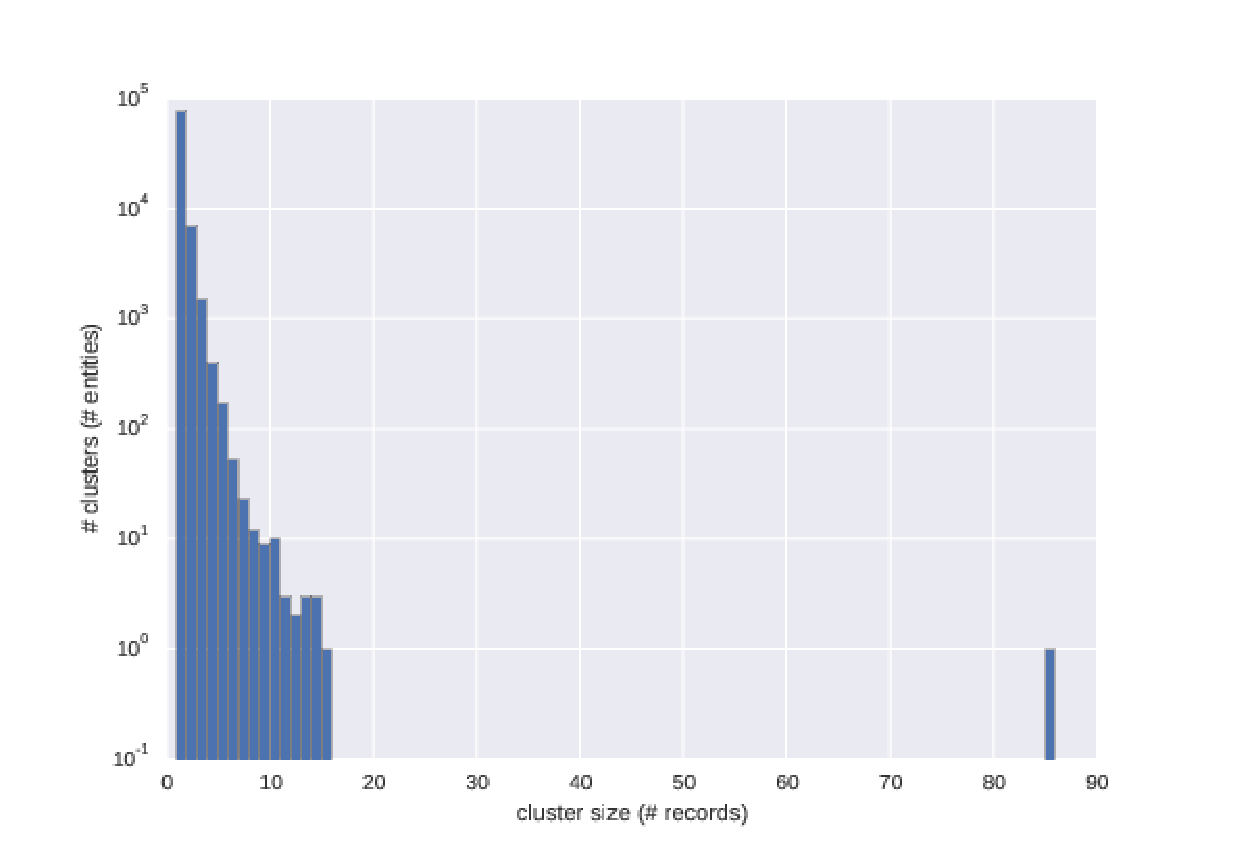
\includegraphics[width=0.15\textwidth]{donors_real.eps}
%      \includegraphics[width=0.3\textwidth]{real_2.pdf}
        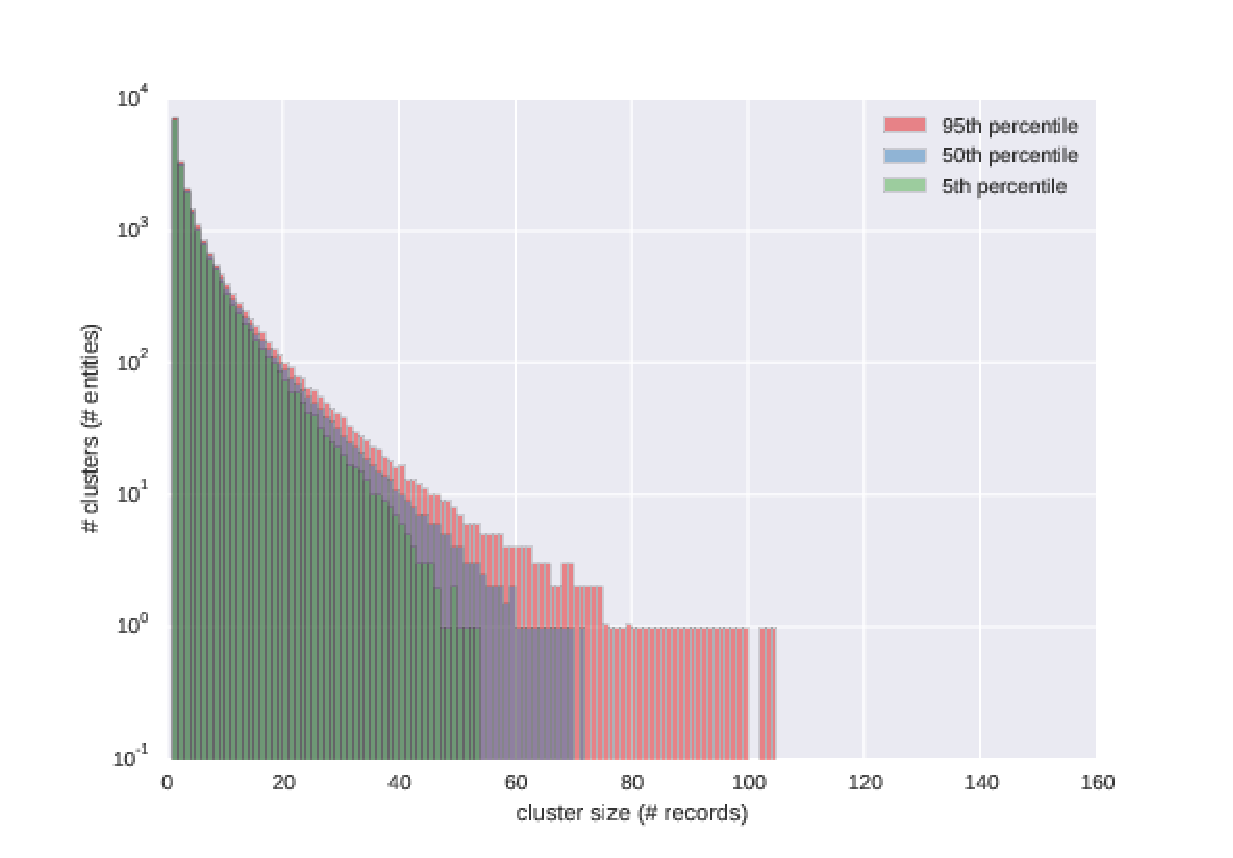
\includegraphics[width=0.15\textwidth]{donors_synthetic.eps}
         \mycaption{Two illustrations of the microclustering problem: (\emph{Left}) a
      histogram of the number of records per entity (i.e., cluster
      sizes) for a database of 100,000 campaign finance donations from
      2011--2012.  \emph{Right}: 
      A histogram of the cluster sizes generated from a Chinese restaurant process simulation with 
      concentration parameter 0.1. }
    \label{fig:small_clustering}
  \end{center}
  
  



\vspace*{1em}

%%% Motivating example
\begin{center}\pbox{0.8\columnwidth}{}{linewidth=2mm,framearc=0.1,linecolor=lightblue,fillstyle=gradient,gradangle=0,
gradbegin=white,gradend=whiteblue,gradmidpoint=1.0,framesep=1em}{\begin{center}{\large \bf Microclustering property }\end{center}}\end{center}
\vspace{.75cm}

\definecolor{myblue}{RGB}{80,80,160}
\definecolor{mygreen}{RGB}{80,160,80}


\begin{center}
\textbf{Traditional Clustering}
\end{center}


\begin{itemize}
\item A number of popular clustering applications assume priors on partitions such as the Dirichlet process and Pitman-Yor process distributions.
\item \emph{Any} infinitely exchangeable partition distribution on the positive integers has a Kingman paintbox representation.
\item Having a Kingman paintbox representation implies that the number of data points in each cluster grows (a.s.) linearly with the total number of data points $N$.
\item By contrast, in entity resolution (and other problems), we expect the size of the clusters to be small even for large datasets.
\end{itemize}

\vspace*{1em}

\begin{center}
\textbf{Microclustering}
\end{center}
A sequence of random partitions $(\Pi_n)_{n=1}^\infty$ satisfies the \emph{microclustering property} if $M_n/n\to0$ in probability as $n\to\infty$, where the size $M_n$ of the largest cluster of $\Pi_n$.

\begin{itemize}
\item Equivalently, $M_n \,/\, n \rightarrow 0$ in probability as $n \rightarrow \infty$.
\item Microclustering requires sacrificing either (i) exchangeability or (ii) self-consistent marginalization of the partitions. 
\item We sacrifice (ii) and assume that $(\sC_1,\sC_2,\dots)$ is an exchangeable sequence of clusters with finite sizes.
\end{itemize}


\vspace{1em}

\begin{center}
  \pbox{0.8\columnwidth}{}{linewidth=2mm,framearc=0.1,linecolor=lightblue,fillstyle=gradient,
    gradangle=0,gradbegin=white,gradend=whiteblue,gradmidpoint=1.0,framesep=1em}{
    \begin{center}
      {\large \bf Exchangeable Sequences of Clusters}
    \end{center}
  }
\end{center}

\vspace*{1em}

We propose a flexible and tractable prior distribution for a random partition that is appropriate for microclustering tasks such as entity resolution.

\begin{itemize}
\item $K$:  number of clusters (random).
\item $\Pi_n=\{C_1,\dots,C_K\}$ is a partition of $[n]$
\item $S_k, \; k=1,\ldots K$: size of the cluster $C_k$. 
\item $z_i, \; n=1,\ldots n$: cluster assignment of the $n$th data point.
\end{itemize}

\vspace*{1em}

A random partition $\Pi_n\sim ESC_{[n]}(P_{\bm{\mu}})$ can be generated as follows.
\begin{enumerate}
\item Conditional on $E_n$, sample $\bm{\mu}\sim P_{\bm{\mu}}$ and $S_1,S_2,\dots|\bm{\mu}\stackrel{iid}\sim\bm{\mu}$. 
\item Define $K$ as the unique positive integer such that $\sum_{j=1}^{K}S_j=n$.
\item Define the cluster allocation variables $(z_1,\dots,z_n)$ as a uniformly at random permutation of the vector
$$(\underbrace{1,\ldots,1}_\text{$S_1$ times},\underbrace{2,\ldots,2}_\text{$S_2$
  times},\ldots\ldots,\underbrace{K,\ldots,K}_\text{$S_K$ times})$$.
\end{enumerate}

where  $\bm{\mu}=(\mu_s)_{s=1}^\infty$, $\mu_s$ is the probability of a cluster of size $s$, $P_{\bm{\mu}}$ is the distribution of  $\bm{\mu}$ and
\begin{equation*}
%E_n=\left\{\exists k \in \N\,\hbox{ such that }\,\sum_{j=1}^k |\sC_j|=n \right\}
E_n=\left\{\hbox{there exists }k \in \N\,\hbox{ such that }\,\sum_{j=1}^k S_j=n \right\}\,.
\end{equation*}
Conditional on the event $E_n$, $K$ is defined as the unique positive integer such that $\sum_{j=1}^{K}S_j=n$.

\vspace*{1em}

\begin{center}
  \pbox{0.8\columnwidth}{}{linewidth=2mm,framearc=0.1,linecolor=lightblue,fillstyle=gradient,
    gradangle=0,gradbegin=white,gradend=whiteblue,gradmidpoint=1.0,framesep=1em}{
    \begin{center}
      {\large \bf Properties of ESC Model}
    \end{center}
  }
\end{center}
\vspace{.65cm}


\begin{center}
\textbf{Prediction Rule}
\end{center}  

Let $\z=(z_1,...,z_n)$ be the cluster allocation variables of $\Pi_n\sim ESC_{[n]}(P_{\bm{\mu}})$.
For any $i=1,\dots,n$, the conditional distribution of $z_i$ given $\z_{-i}=\z\backslash z_i$ and $\bm{\mu}$ is
%The corresponding prediction rule is given by
\begin{equation*}\label{eq:prediction_rule_conditional}
\P(z_i=j|\z_{-i},\bm{\mu})
\propto
\left\{
\begin{array}{ll}
(s_j+1)
\frac{\mu_{(s_j+1)}}{\mu_{s_j}}& \hbox{if }j=1,\dots,k_{-i},
\\
(k_{-i}+1)\mu_1 & \hbox{if }j=k_{-i}+1\,,
\end{array}
\right.
\end{equation*}
where %$\z=(z_1,...,z_n)$ are the cluster allocation variables, 
%$\z_{-i}=\z\backslash z_i$ and 
$k_{-i}$ is the number of clusters in $\z_{-i}$.

\vspace{.65cm}

\begin{center}
\textbf{Number of clusters}
\end{center}  

 Assume $\sum_{s=1}s\mu_s< \infty$ and let $K_{n}$ be the number of clusters of $\Pi_n$.
%a random partition $\Pi_n\sim ESC_{[n]}(\bm{\mu})$.
As $n\rightarrow\infty $ it holds
\begin{align*}\label{eq:limit_K}
\frac{K_n}{n}&\stackrel{p}\rightarrow \left(\sum_{s=1}^\infty s\mu_s\right)^{-1}\,,
\end{align*}
where $\stackrel{p}\rightarrow$ denotes convergence in probability.

This implies that, if the mean of $\bm{\mu}$ is finite (i.e.\ $\sum_{s=1}^\infty s\mu_s< \infty$) the number of clusters of $\Pi_n$ grows linearly with the number of data points $n$.
 
\vspace{.65cm}
 
\begin{center}
\textbf{Proportion of clusters of given size}
\end{center}  

 Assume $\sum_{s=1}s\mu_s< \infty$.
\begin{enumerate}
\item[(a)] Let $M_{s,n}$ be the number of clusters of size $s$ in $\Pi_n$. 
As $n\rightarrow\infty $
$$
\frac{M_{s,n}}{n}\stackrel{p}\rightarrow \frac{\mu_s}{\sum_{\ell=1}^{\infty}\ell\mu_\ell}\,.
$$
\item[(b)] 
The size $S_j$ of a cluster chosen uniformly at random from the clusters of $\Pi_n$ converges in distribution to $\bm{\mu}$ as $n\rightarrow\infty $.
\end{enumerate}
This implies that, asymptotically, the distribution of the size of a randomly chosen cluster from $\Pi_n$ coincides with $\bm{\mu}$ 
%which provides a natural interpretation for such a parameter.
%This allows one to specify appropriate prior distributions for $\Pi_n$, by incorporating into $P_{\bm{\mu}}$ any knowledge about the expected behavior of the sizes of the clusters of $\Pi_n$, and also 
%to extract meaningful information from the posterior distribution of $\bm{\mu}$.
 
\vspace*{1em}

\begin{center}
  \pbox{0.8\columnwidth}{}{linewidth=2mm,framearc=0.1,linecolor=lightblue,fillstyle=gradient,
    gradangle=0,gradbegin=white,gradend=whiteblue,gradmidpoint=1.0,framesep=1em}{
    \begin{center}
      {\large \bf Model Specification}
    \end{center}
  }
\end{center}
\vspace{.65cm}
 
 
\begin{center}
\textbf{ESC-NB Model}
\end{center}  
  
%We assume $\bm{\mu}=(\mu_s)_{s=1}^\infty$ to have a parametric form.

We model $\bm{\mu}$ as a Negative Binomial distribution truncated on $\{1,2,\dots\}$, $\bm{\mu}=NegBin(r,p)$, meaning that, for all $s=1,2,\dots$; $\mu_s$ is the following deterministic function of $r$ and $p$
\begin{equation*}\label{eq:mu_esc_NB}
\mu_s(r,p)=\gamma\frac{\Gamma(s+r)p^s }{\Gamma(r)s!}\,,
\end{equation*}
where $\gamma=\frac{(1-p)^{r}}{1-(1-p)^r}$.
 
   
\begin{center}
\textbf{ESC-D Model}
\end{center}  

A more flexible choice is to assume $\bm{\mu}\sim Dir(\alpha,\bm{\mu}^{(0)})$, where $\bm{\mu}^{(0)}=(\mu^{(0)}_s)_{s=1}^\infty$ is a sequence of non-negative numbers satisfying $\sum_{s=1}^\infty\mu^{(0)}_s=1$.
We then impose a parametric form on $\bm{\mu}^{(0)}$ in an analogous way to the ESC-NB model.

\vspace*{1em}

\begin{itemize}
\item $r>0$ and $p\in(0,1)$ are given prior distributions, $r\sim Gamma(\eta_r,s_r)$ and $p\sim Beta(u_p,v_p)$.
\item The hyperparameters $\eta_r$, $s_r$, $u_p$ and $v_p$ are chosen to reflect the prior expectations on the distribution of the cluster sizes $S_j$.
\end{itemize}


\vspace*{1em}

\vspace{.25cm}\begin{center}\pbox{0.8\columnwidth}{}{linewidth=2mm,framearc=0.1,linecolor=lightblue,
fillstyle=gradient,gradangle=0,gradbegin=white,gradend=whiteblue,gradmidpoint=1.0,framesep=1em}
{\begin{center}{\large \bf Entity Resolution Model}\end{center}}\end{center}\vspace{.3cm}
\vspace*{1em}

The observed data $\x = (x_1,\dots,x_n)$ consist of $n$ records and each record $x_i$ contains $L$ fields $(x_{i\ell})_{\ell=1}^L$. We assume that fields within clusters are independent and each of them depends only on the following field specific parameters: 
\begin{itemize}
\item a distortion probability $\beta_\ell\in(0,1)$ that reflects the proneness to errors of each field, and
\item a density vector $\btheta_{\ell}=(\theta_{\ell d})_{d=1}^{D_\ell}\in[0,1]^{D_\ell}$ that characterizes the distribution of categories per field, where $\sum_{d=1}^{D_\ell}\theta_{\ell d}=1$. 
\end{itemize}


Let $y_{j\ell}$ represent the true $\ell$-th feature of the entity associated to cluster $C_j \in \Pi_n$ for $j=1,\ldots, K$, and  $\zeta(\Pi_{n}, i)$ be a function that maps record $i$ to its latent cluster assignment $z_i$ according to 
$\Pi_{n}$. 

The microclustering model for entity resolution is as follows: 
\begin{center}
\vspace*{-1em}
\begin{align}
x_{i\ell} | y_{j\ell}, \zed, \btheta_{\ell}, \beta_{\ell}  &\stackrel{iid}\sim \beta_{\ell}\btheta_{\ell} + (1-\beta_{\ell})\delta_{y_{z_i\ell}} \label{eq:x_giv_y}\\
y_{j\ell} & \stackrel{iid}{\sim} \btheta_{\ell}  \label{eq:y_gen} \\
\zed & = \zeta(\Pi_{n}, i)  \\
\Pi_n & \sim ESC_{[n]}(\bm{\mu})
\end{align}
\end{center}
where $\delta_{y}$ is the Dirac-delta function at $y$, and $\btheta_{\ell}$ is fixed and assumed to be the empirical distribution of the data.

\vspace*{1em}

\vspace{.25cm}\begin{center}\pbox{0.8\columnwidth}{}{linewidth=2mm,framearc=0.1,linecolor=lightblue,
fillstyle=gradient,gradangle=0,gradbegin=white,gradend=whiteblue,gradmidpoint=1.0,framesep=1em}
{\begin{center}{\large \bf Chaperones Algorithm}\end{center}}\end{center}\vspace{.3cm}
\vspace*{1em}

If we let $c_i \in \Pi_n$ denote the cluster containing
element $i$, then each iteration consists of: 
\begin{enumerate}[label=\textbf{\arabic*.}]
\item Randomly choose two \emph{chaperones}, $i, j \in \{1, \ldots,
  n\}$ from a distribution $P(i, j \g x_1, \ldots, x_n)$ where the
  probability of $i$ and $j$ given $x_1, \ldots, x_n$ is greater
  than zero for all $i \neq j$. This distribution must be
  independent of the current state of the Markov chain $\Pi_n$;
  however, crucially, it may depend on the observed data points
  $x_1, \ldots, x_n$.

\item Reassign each element $k \in c_i \cup c_j$ by sampling from $P(\Pi_n \g n,
  \Pi_n \!\setminus\! k, c_i \cup c_j, x_1, \ldots, x_n)$.
\end{enumerate}

\vspace*{0.5em}

Step 2 is almost identical to the restricted
Gibbs moves found in existing split-merge algorithms (Jain and Neal, 2004), except that the chaperones $i$ and $j$ can also
change clusters, provided they do not abandon any of their children.
\vspace*{1em}

%\begin{center}
%\includegraphics[width=0.13\textwidth]{chaperones1}
%\end{center}
%\begin{center}
%\includegraphics[width=0.13\textwidth]{chaperones2}
%\end{center}
%\begin{center}
%\includegraphics[width=0.13\textwidth]{chaperones3}
%\end{center}
%\begin{center}
%\includegraphics[width=0.13\textwidth]{chaperones4}
%\end{center}





%\begin{center}
%\includegraphics{chaperones_v3.eps}
%\end{center}


\vspace{.25cm}\begin{center}\pbox{0.8\columnwidth}{}{linewidth=2mm,framearc=0.1,linecolor=lightblue,
fillstyle=gradient,gradangle=0,gradbegin=white,gradend=whiteblue,gradmidpoint=1.0,framesep=1em}
{\begin{center}{\large \bf Application}\end{center}}\end{center}
\vspace*{1em}

%\begin{center}
%\textbf{Assessing Model Fit}
%\end{center}
%\begin{itemize}
%\item We compare the NBNB and PERPS to several
%commonly used infinitely exchangeable models.
%%: mixtures of
%%finite mixtures (MFM)~\cite{miller15mixture}, DP mixtures, and PYP
%%mixtures. 
%\item We assess how well each model ``fits'' partitions typical of
%those arising in entity resolution and other tasks involving clusters
%whose sizes grow sublinearly with $N$.
%\item For simplicity and interpretability, we define
%the best parameter values for each model to be the values that
%maximize the probability of the observed partition.
%%\item We use two observed partitions -- ones simulated and one real. 
%\end{itemize}

\begin{center}
\textbf{The Data}
\end{center}

\begin{itemize}
\item Social Diagnosis Survey (SDS): panel study of objective and subjective quality of life in Poland focused on individuals aged 16 and above. 
\item  We take a subsample of $n=10,000$ records from the survey waves in the years 2011, 2013, and 2015. 
\item The true number of clusters in the datasets is $K= 5,505$ with 2,505 singleton clusters, 1,505 clusters of size two, and 1,495 clusters of size three.
\item We use the fields of sex, date of birth (day, month and year), province of residence, and education level.
\end{itemize}

\begin{center}
\textbf{Results}
\end{center}

\begin{center}
\includegraphics[width=0.15\textwidth]{poland/Kpost_poland10k_nostat_ParChapTrunc1p}
\vspace{-1cm}
\includegraphics[width=0.15\textwidth]{poland/Kpost_poland10k_nostat_ParChapTrunc5p}
\vspace{-1cm}
\includegraphics[width=0.3\textwidth]{poland/Stats_poland10k_nostat_ParChapTrunc}
\mycaption{Top: Posterior distributions of the number of clusters for DP, PY, ESC-NB and ESC-D models truncating the prior distribution of the distortion probabilities at $c=0.01$ (top left) and $c=0.05$ (top right) for SDS subsample dataset of $n=10,000$ records. Bottom: Side-by-side boxplots of the posterior distributions of the number of singleton clusters, max, mean and 90th percentile of cluster sizes for all models and truncation values. The red vertical lines (top) and gray dashed horizontal lines (bottom) represent the true statistic values. The ESC-NB and ESC-D models with truncation value of $c=0.05$, ESC-NB(0.05) and ESC-D(0.05), capture the true partition statistics and show the best performance.} 
\end{center}

\vspace{.25cm}\begin{center}\pbox{0.8\columnwidth}{}{linewidth=2mm,framearc=0.1,linecolor=lightblue,
fillstyle=gradient,gradangle=0,gradbegin=white,gradend=whiteblue,gradmidpoint=1.0,framesep=1em}
{\begin{center}{\large \bf Discussion}\end{center}}\end{center}
\vspace*{1em}

\begin{itemize}
\item We overcome major limitations in the existing literature for microclustering models -- a lack of interpretability, identifiability, and full characterization of the model asymptotic properties.
\item The resulting framework offers great flexibility in terms
of the prior distribution of cluster sizes, is computationally tractable and suitable
for general microclustering tasks. 
\item The theoretical results
allow to devise simple and efficient Markov chain Monte Carlo algorithms to perform
statistical inference. 
\item Extensions to include string features in the entity resolution model.
\end{itemize}

\textbf{Acknowledgements}: This work was supported in
part by NSF Big Data Privacy, NSF Career and the
Foerster-Bernstein Postdoctoral Fellowship.

%\vspace*{-3em}
%\tiny{
\scriptsize{
\bibliographystyle{ims}
\bibliography{references}
}
\phantom{.}
\end{multicols}



\end{poster}

\end{document}

% \includegraphics{plots/band1.eps}
%      \includegraphics{plots/band2.eps}
%      \includegraphics{plots/band3.eps}\\
%      \includegraphics{plots/band4.eps}
%      \includegraphics{plots/band5.eps}
%      \includegraphics{plots/band6.eps}\\
%      \includegraphics{plots/band7.eps}
%      \includegraphics{plots/band8.eps}\\
%      \includegraphics{plots/legend1.eps}
%      \mycaption{Medians (smooth lines) and $95\%$ probability bands (shaded regions around the medians) of the posterior distributions of the main effects of the LCM at 8 different MODIS bands.}
      


